\documentclass{beamer}
\usepackage{csvsimple,booktabs}
\usepackage{tabularx}
\usepackage[utf8]{inputenc}
%\usepackage{csvsimple,booktabs}

%\usepackage{tabularx}
\usepackage{graphicx}
\usepackage{geometry}

\usetheme{Madrid}
\useoutertheme{split} % Alternatively: miniframes, infolines, split
\useinnertheme{circles}

\definecolor{UBCblue}{rgb}{0.04706, 0.13725, 0.26667} % UBC Blue (primary)
\definecolor{UBCgrey}{rgb}{0.3686, 0.5255, 0.6235} % UBC Grey (secondary)
% \definecolor{peyaj1}{rgb}{0.4705, 0.4549, 0.9294}
% \definecolor{peyaj2}{rgb}{0.6588, 0.8431, 0.9411}

\setbeamercolor{palette primary}{bg=UBCblue,fg=white}
\setbeamercolor{palette secondary}{bg=UBCblue,fg=white}
\setbeamercolor{palette tertiary}{bg=UBCblue,fg=white}
\setbeamercolor{palette quaternary}{bg=UBCblue,fg=white}
\setbeamercolor{structure}{fg=UBCblue} % itemize, enumerate, etc
\setbeamercolor{section in toc}{fg=UBCblue} % TOC sections

% Override palette coloring with secondary
\setbeamercolor{subsection in head/foot}{bg=UBCgrey,fg=white}

\title{Report of Analysis on BDjobs Data(2016 - 2021)}
\author{SrJ}
\date{\today}

\newcommand{\generateframe}[2]{
	\begin{frame}{#2}
		\begin{table}[!htb]
			\centering
			\caption{#2}
			\label{tab:#2}
			\csvautobooktabular{"Tables/#1.csv"}
		\end{table}
	\end{frame}
}

\begin{document}
	\begin{frame}{Start}
		\maketitle
	\end{frame}

	\generateframe{emp_type}{Type of Employment}
	\generateframe{pos_level}{Position Level}
	\generateframe{gender}{Gender}
	\generateframe{location}{Location}
	\generateframe{industry}{Industry}
	\tiny{
	\generateframe{title_rank}{Job Rank}
	\generateframe{supply_demand}{Supply Demand}
	\begin{frame}
	\begin{figure}
		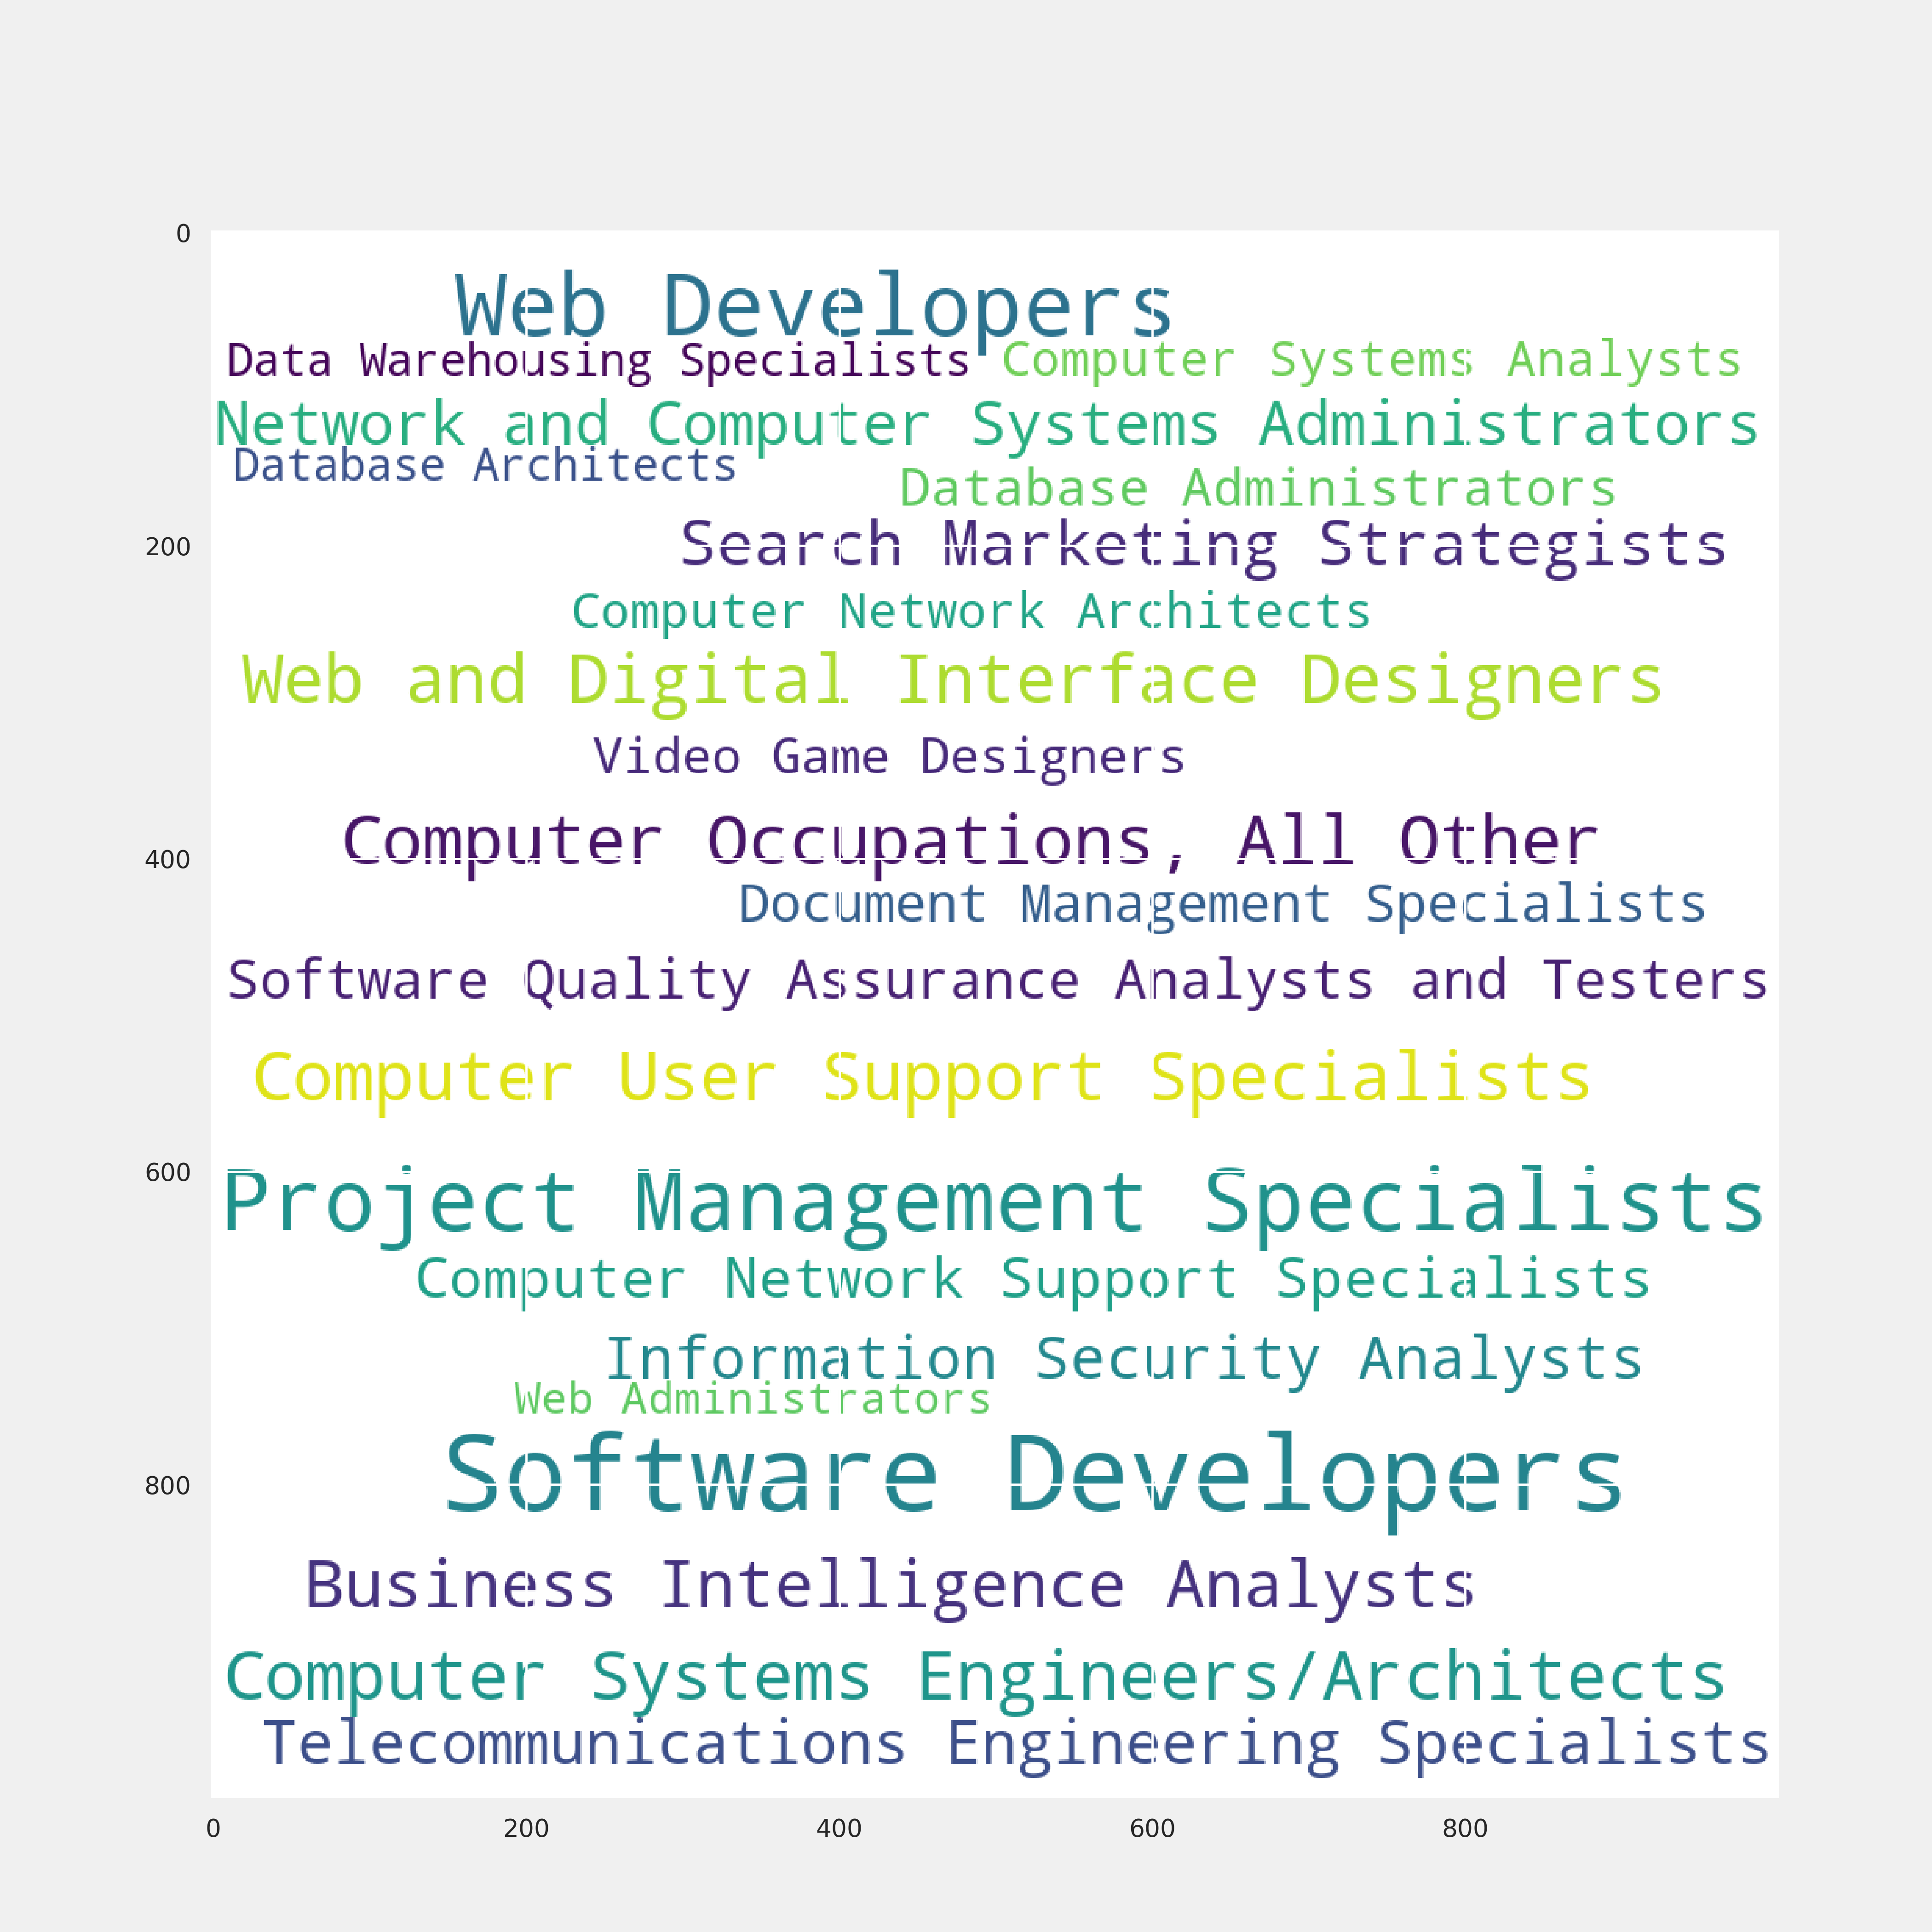
\includegraphics[scale=0.25]{WordCloud.png}
		\caption{OSC-ONET Job Title}
	\end{figure}
	\end{frame}


\end{document}